\chapter{Results}
    In this chapter we present our results for the implementation of our pose estimation and the depth map acquired from \citetitle{luo2020consistent}~\cite{luo2020consistent}.
    We try to pinpoint the problems we encountered in our pipeline by comparing our results to the synthetic dataset 'lr kt2' from \citetitle{handa:etal:ICRA2014}~\cite{handa:etal:ICRA2014}.
    \section{pose optimization}
        Figure~\ref{fig:initial_reconstruction} shows our first valid results for one of our own videos.
        We were hoping to drastically improve on this results after optimizing the global poses.
        \begin{figure}[ht]
            \centering
            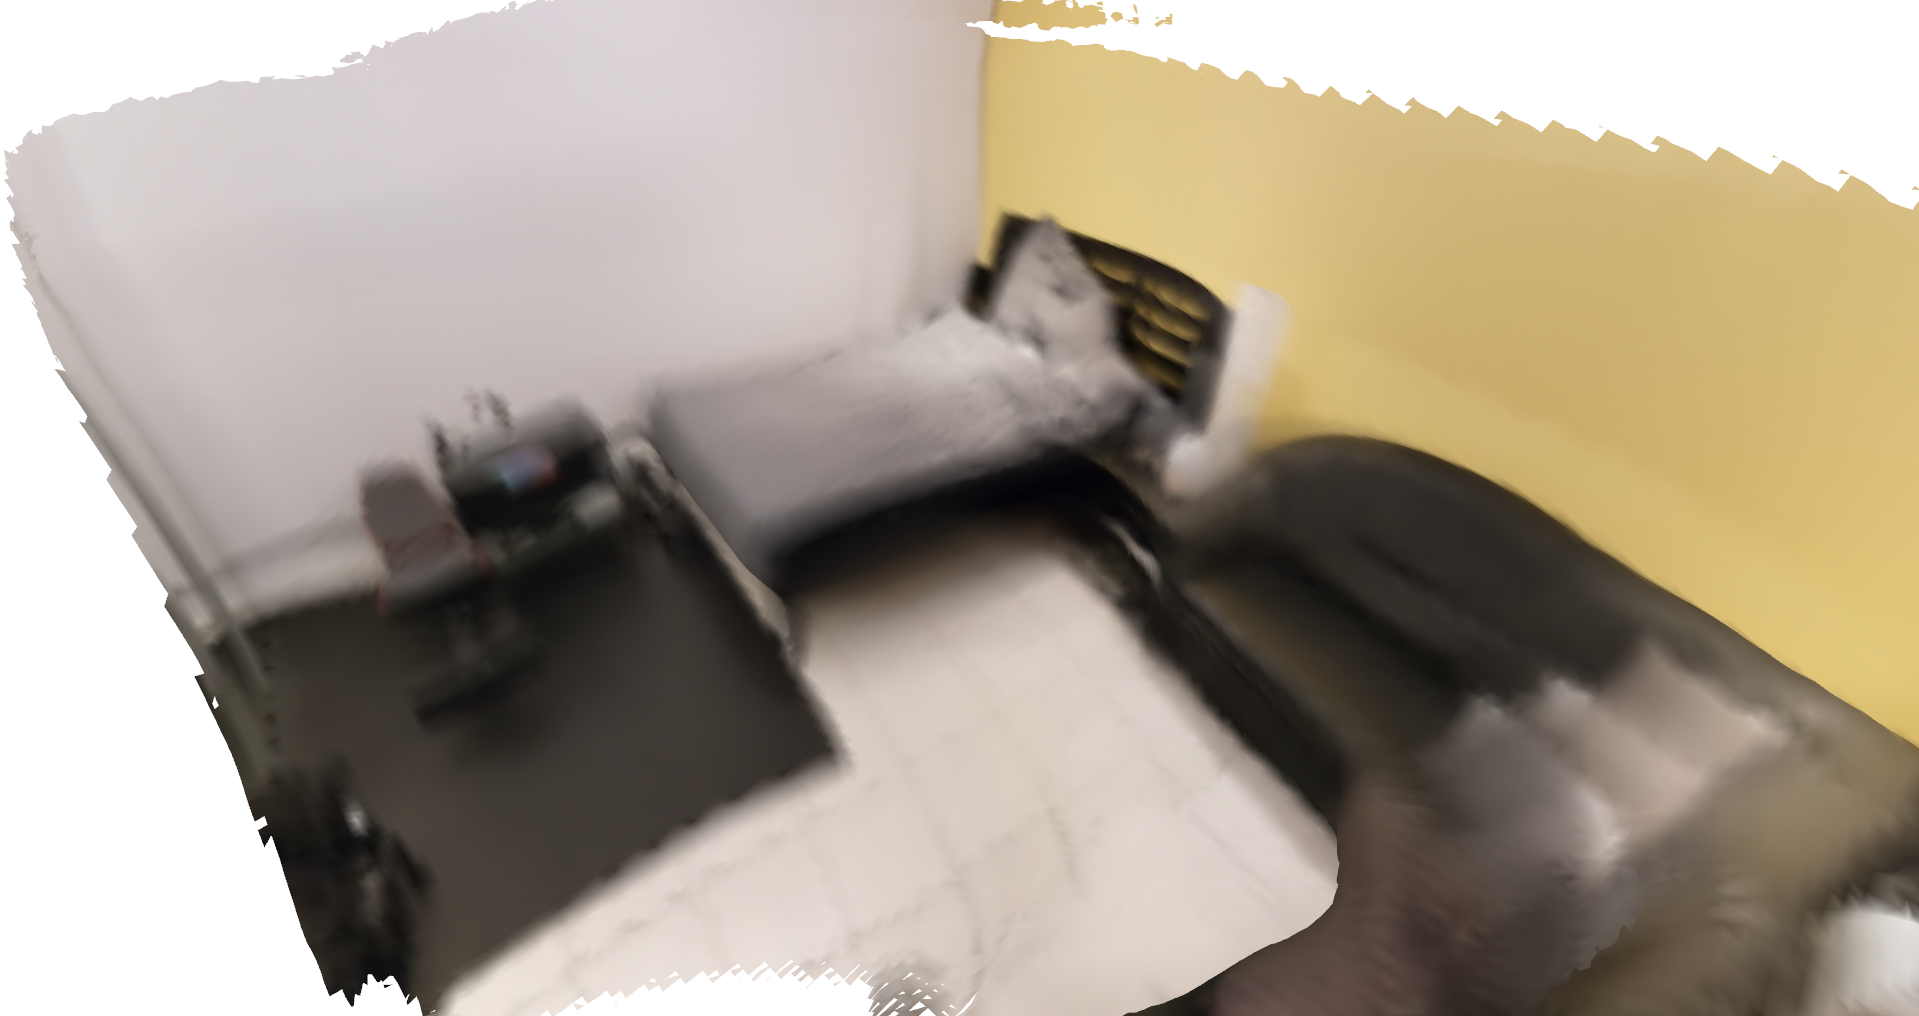
\includegraphics[width=.6\textwidth]{images/initial_reconstruction.png}
            \caption{Initial reconstruction on unoptimized pose estimates on one of our own videos.}
            \label{fig:initial_reconstruction}
        \end{figure}\\
        It turned out that our method for the pose estimation, described in chapter~\ref{sec:method_pose_optimization}, while not meant to be fast, was actually very computationally expensive.
        As the amount of frames increases, the number of valid frame pairs can potentially grow exponentially.
        In order to avoid computing for unreasonable amounts of time, we used a similar method to reduce the computational effort as described in \citetitle{dai2017bundlefusion}~\cite{dai2017bundlefusion}.
        While They use a hierarchy to condense the information within one chunk of 11 frames into one keyframe, we simply selected our keyframes without using the information of the remaining frames.\\
        As we could not identify a visible improvement after the pose optimization, we ran everything on the synthetic dataset 'lr kt2' from \citetitle{handa:etal:ICRA2014}~\cite{handa:etal:ICRA2014}.
        With the ground truth of the extrinsics we were able to properly compare our initial poses to the optimized poses.
        To compare extrinsics from different coordinate systems we needed to find a transform to match the trajectories.
        This transform includes rotation, scaling, and translation.
        One option is to simply align the poses of the first frame.
        While this is a trivial method, it does not lead to a satisfying alignment and makes it really hard to find the proper scale.
        Results of this alignment are shown in figure~\ref{sfig:align_first_pair}.\\
        We can observe that the alignment is not satisfactory.
        Employing a method like ICP (iterative closest point) achieves a much better alignment.
        We implemented an error function for the deviation of the two trajectories that takes 7 unknowns: three angles for the rotation $R$, three variables for the translation $t$, and one unknown for the scale $s$:
        \begin{equation*}
            E_{\text{alignment}}(R,t,s) =
            \sum_{i=0} \left[
                q_i - s \times Rp_i - t
            \right]^2
            \label{eq:ealign}
        \end{equation*}
        Where $q_i$ is point $i$ of the target trajectory and $p_i$ is point $i$ of the trajectory that is transformed.
        With this error function we again used scipy.optimize.minimize to obtain the optimal transform.
        The results are displayed in figures~\ref{sfig:align_global}~\&~\ref{sfig:align_global_opt}\\
        \begin{figure}[ht]
            \centering
            \begin{subfigure}[b]{.32\textwidth}
                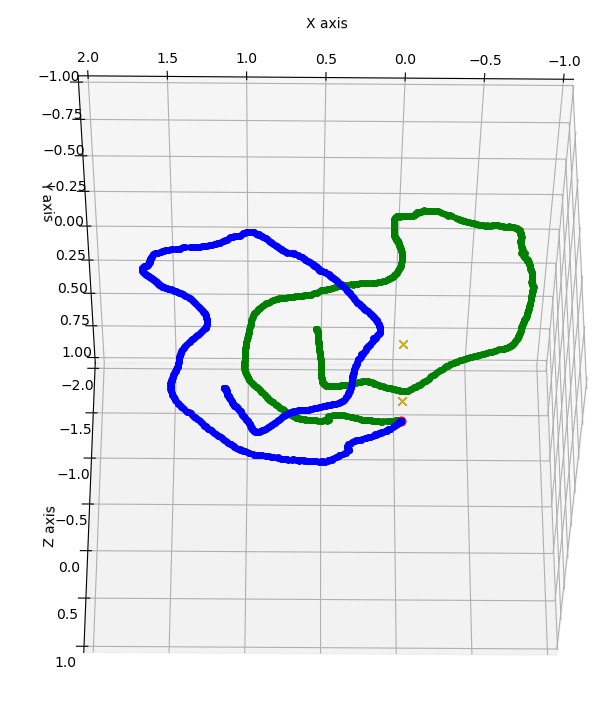
\includegraphics[width=.95\textwidth]{images/align_first_pair}
                \caption{Aligning two trajectories by aligning the first pose of both.}
                \label{sfig:align_first_pair}
            \end{subfigure}
            \begin{subfigure}[b]{.32\textwidth}
                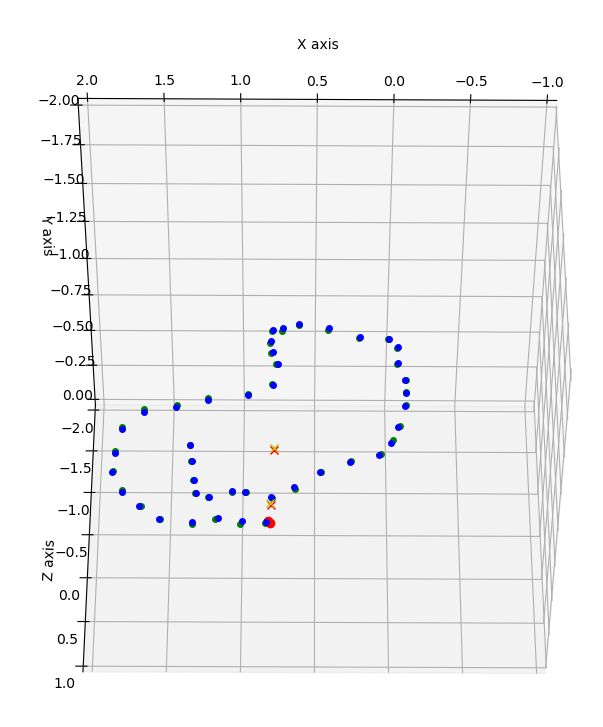
\includegraphics[width=.95\textwidth]{images/align_global}
                \caption{ICP-like global alignment of unoptimized extrinsics}
                \label{sfig:align_global}
            \end{subfigure}
            \begin{subfigure}[b]{.32\textwidth}
                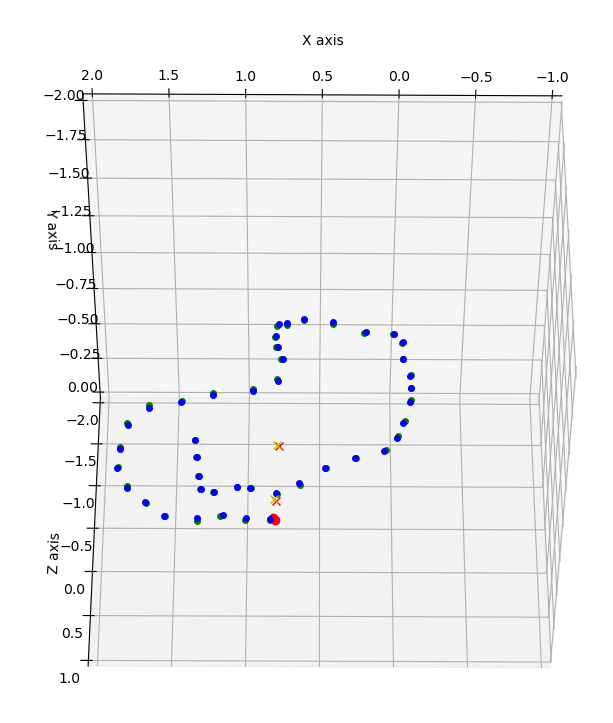
\includegraphics[width=.95\textwidth]{images/align_global_opt}
                \caption{ICP-like global alignment of optimized extrinsics}
                \label{sfig:align_global_opt}
            \end{subfigure}
            \caption[]{\ref{sfig:align_first_pair} aligning both initial poses perfectly. \ref{sfig:align_global} ICP-like global alignment of unoptimized extrinsics. \ref{sfig:align_global_opt} ICP-like global alignment of optimized extrinsics. For both trajectories the orientation of the first pose is indicated by two crosses into the direction the camera is facing, red for ground truth and yellow for the other trajectory. \ref{sfig:align_global}~\&~\ref{sfig:align_global_opt} were reduced with a stride of 20.}
            \label{fig:traj_alignment}
        \end{figure}\\
        While the cost function described in equation~\ref{eq:edense} provides a lower cost for the optimized extrinsics, the alignment error from equation~\ref{eq:ealign} was actually higher than the unoptimized extrinsics.
        So the optimized poses actually fir worse to the ground truth than the initial estimates:
        \begin{center}
            \begin{tabular}[]{c | c | c}
                & unoptimized poses & optimized poses\\
                \hline
                $E_{\text{dense}}$ & $1.7203$ & $1.6081$\\
                \hline
                $E_{\text{alignment}}$ & $1.2420\times10^{-2}$ & $1.2998\times10^{-2}$
            \end{tabular}
        \end{center}
        As the optimized extrinsics also showed little to no improvement to the 3D reconstruction we analyzed the quality of our depth estimates.
    \section{Consistent Depth}
        Once we started testing on the ground truth dataset we were able to compare all possible combinations of extrinsics and depth maps and compare.
        Figure~\ref{sfig:corner} displays the difference between the ground truth depth and the depth map from \citetitle{luo2020consistent}.
        We overlayed a full reconstruction of the ground truth with one image using our depth map.
        We can clearly observe the left and upper corner of the room being slightly curved, but very far from the 90\textdegree angle that they are supposed to form.
        Comparing figures~\ref{sfig:depth_ours}~\&~\ref{sfig:depth_truth}, we can observe that our depth estimate simply does not come close to the ground truth.\\
        \begin{figure}[ht!]
            \centering
            \begin{subfigure}[b]{.49\textwidth}
                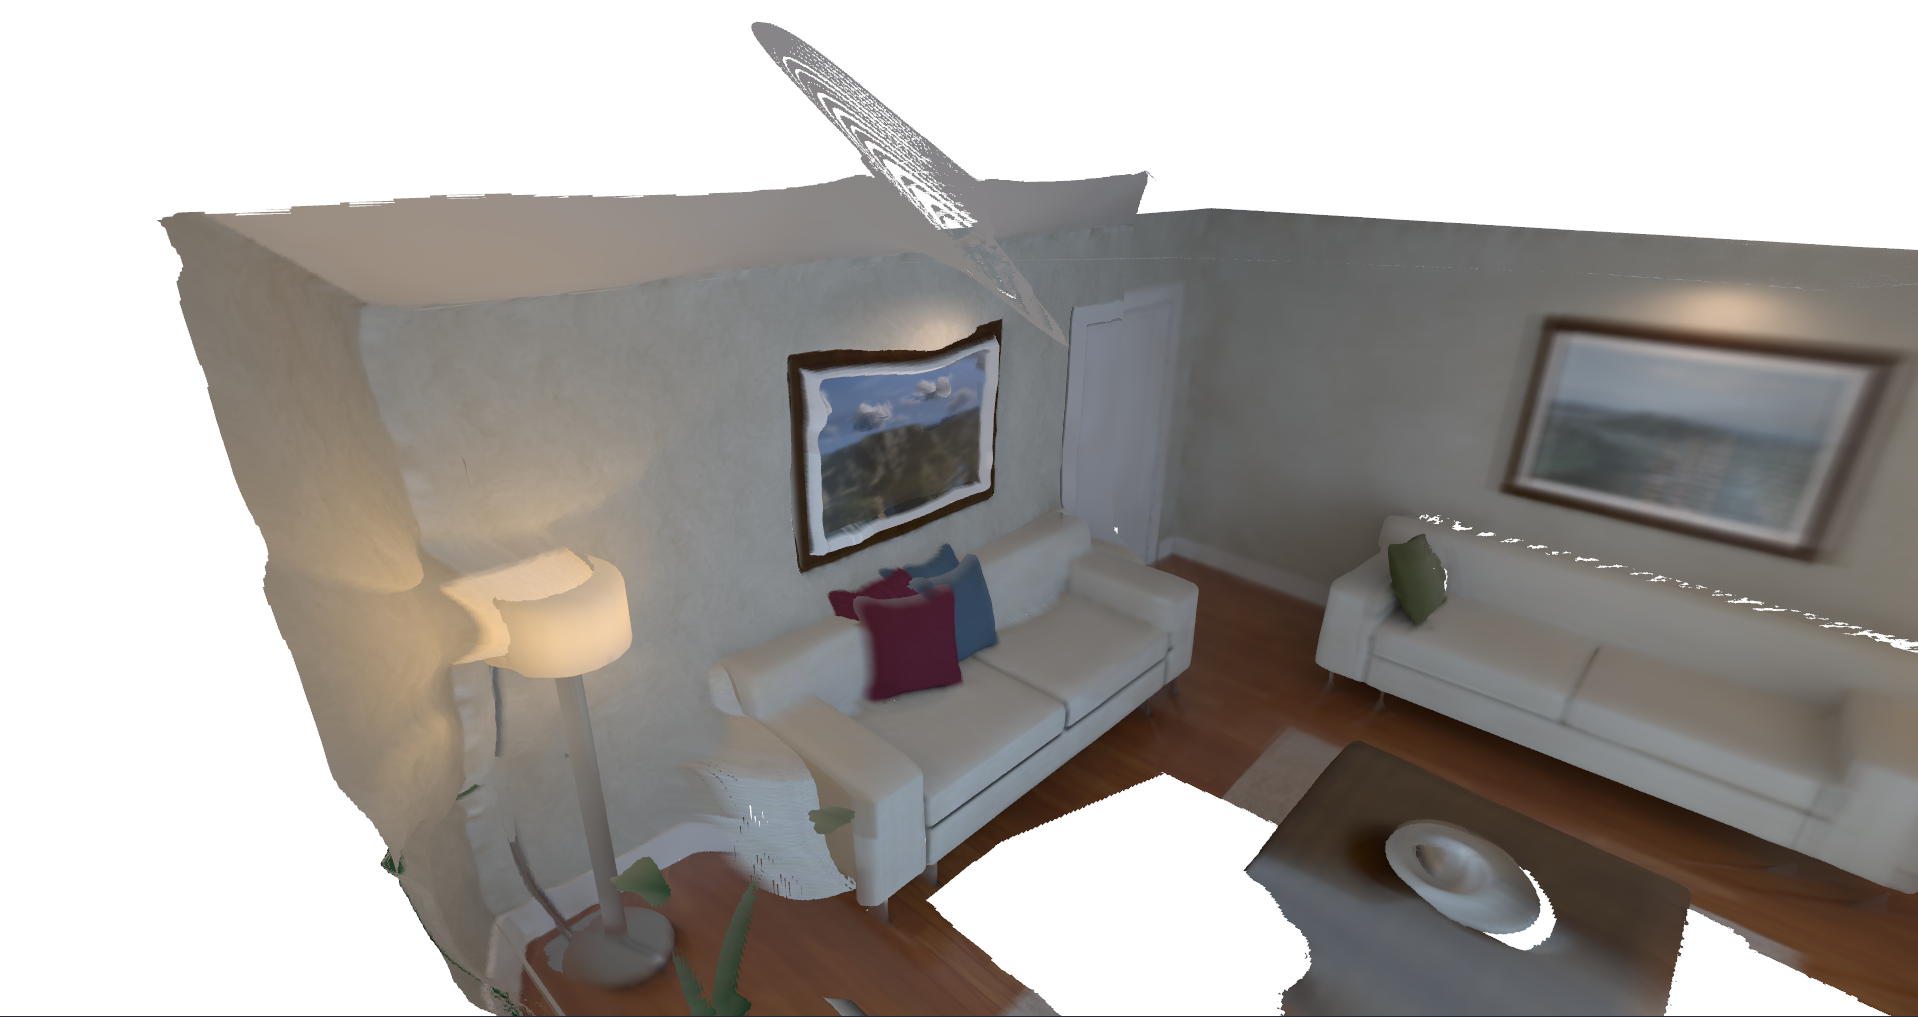
\includegraphics[width=\textwidth]{images/depth_corner}
                \caption{One frame from our depth is overlayed with a full reconstruction using the ground truth depth, corners seem round with our depth.}
                \label{sfig:corner}
            \end{subfigure}\\
            \begin{subfigure}[b]{.49\textwidth}
                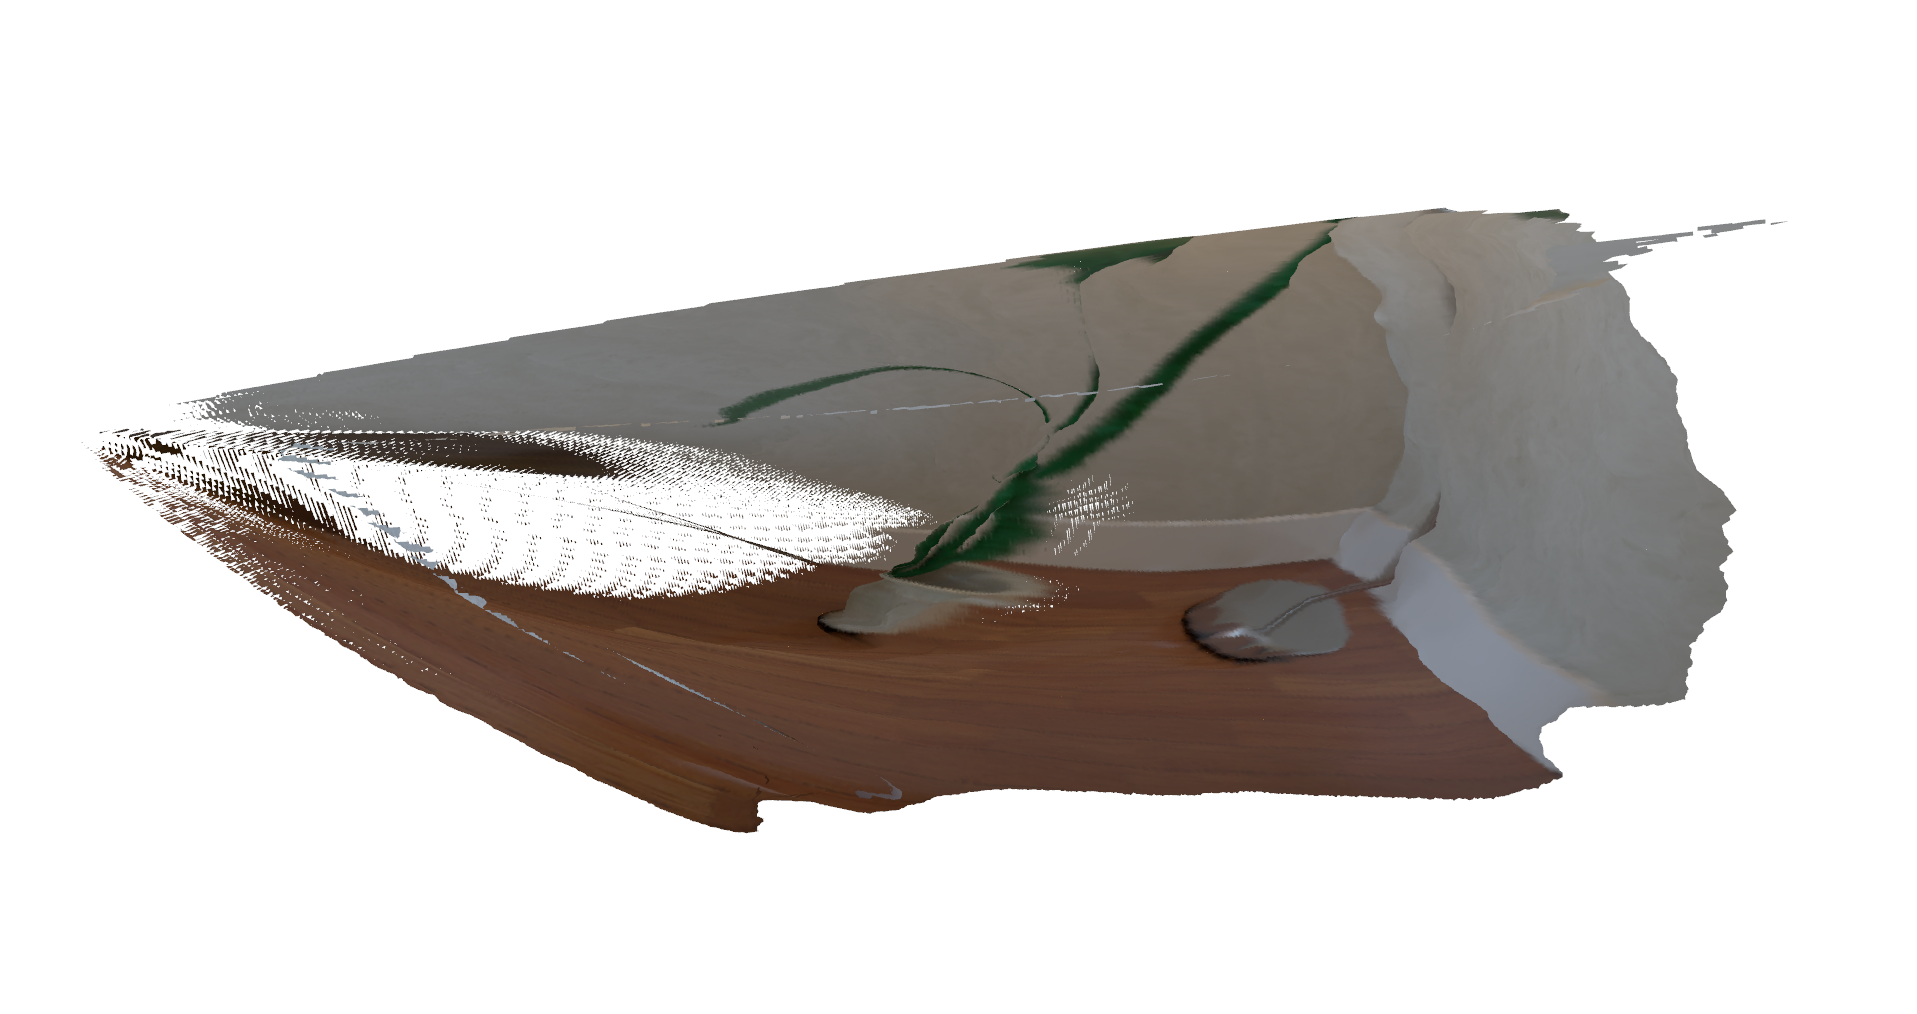
\includegraphics[width=\textwidth]{images/depth_ours}
                \caption{Single frame reconstruction of one of the frames towards the end of the video using our depth.}
                \label{sfig:depth_ours}
            \end{subfigure}
            \begin{subfigure}[b]{.49\textwidth}
                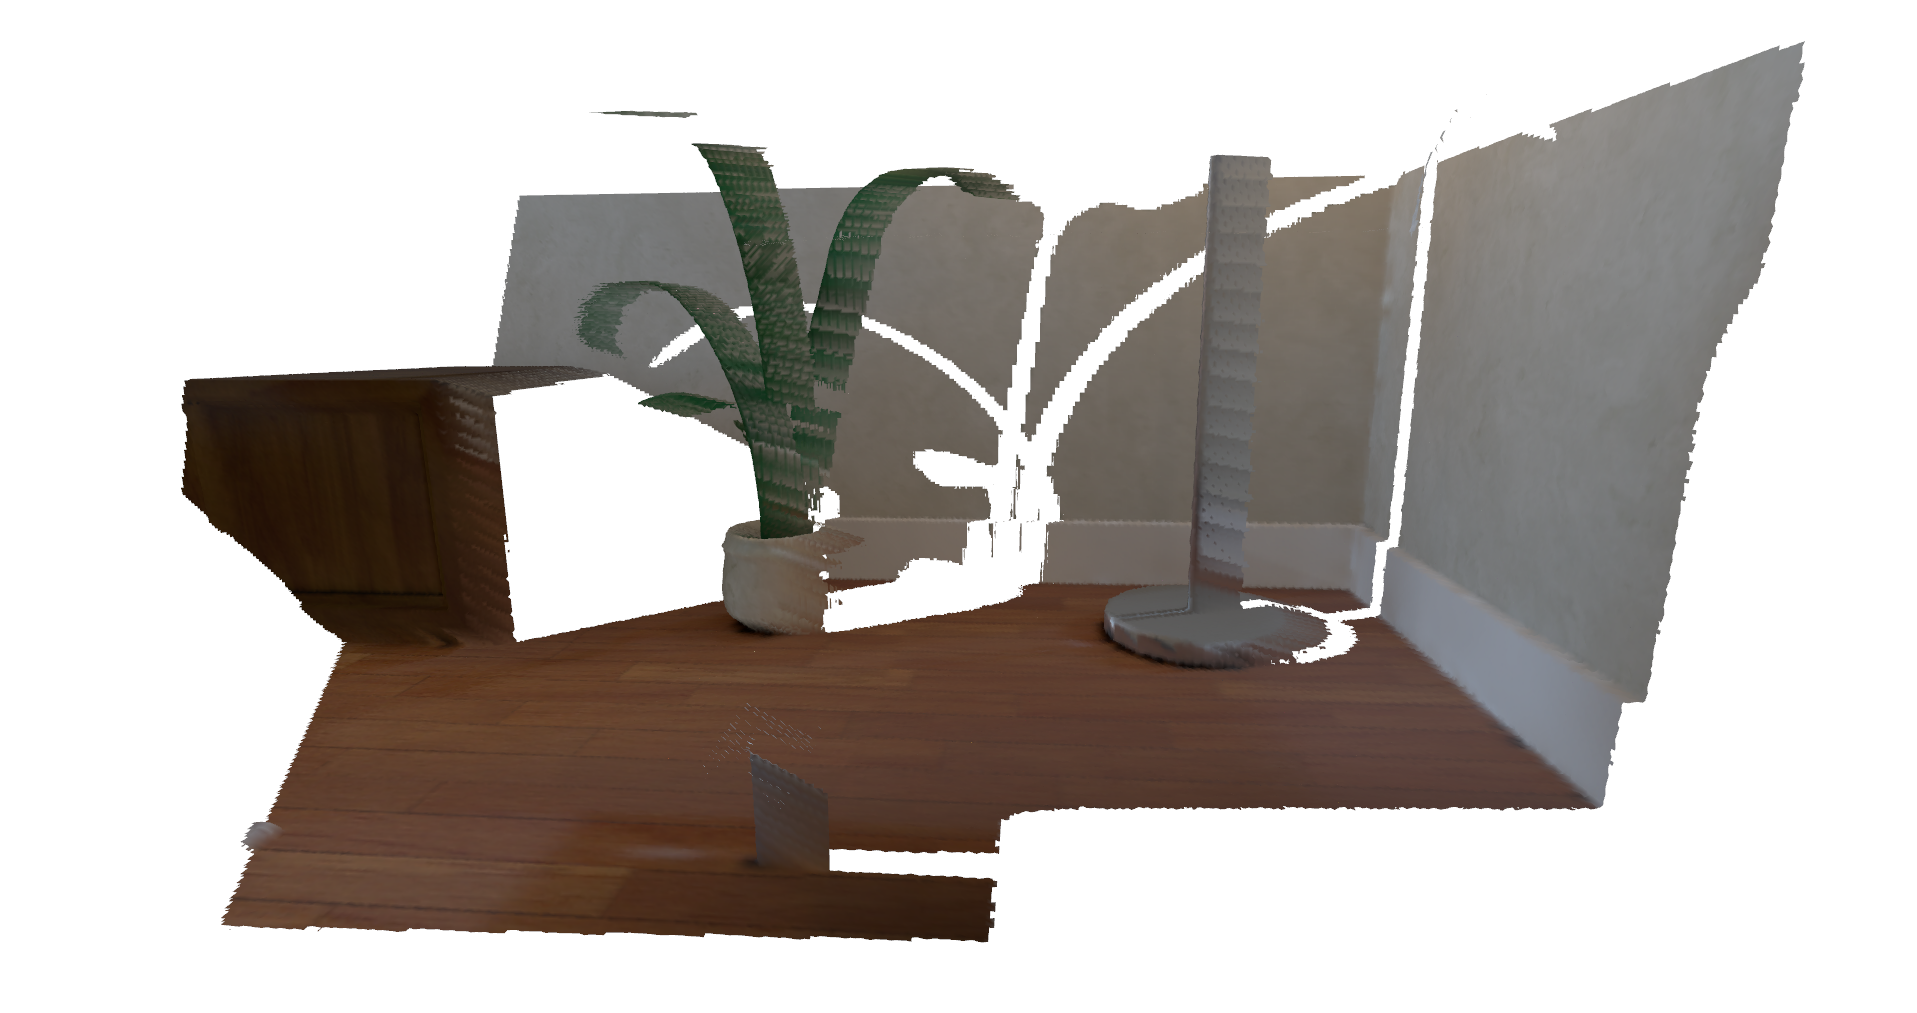
\includegraphics[width=\textwidth]{images/depth_truth}
                \caption{Single frame reconstruction of one of the frames towards the end of the video using the ground truth depth.}
                \label{sfig:depth_truth}
            \end{subfigure}
            \caption{Visual comparison between our depth and the ground truth. In \ref{sfig:depth_ours}~\&~\ref{sfig:depth_truth} only single frames were used for the reconstruction.}
            \label{fig:depth_comparisson}
        \end{figure}\\
        \newpage
        We also investigated the depth discrepancy by producing videos for both depths and comparing them at specific times.
        For interesting frames we compared them and visualizing the error as a heatmap.
        This endeavor required us to scale one of the depth maps to fit with the other.
        We tried to minimize the sum, median, and mean of the error in an attempt to find the best scale to use.
        Two error heatmaps and their respective RGB frames are shown in figure~\ref{fig:depth_error}.
        We chose a diverging colormap to visualize if the error is negative or positve.
        Blue indicates that our depth is lower than the ground truth, red indicates that our depth is higher.
        \begin{figure}[ht]
            \centering
            \begin{subfigure}[b]{.48\textwidth}
                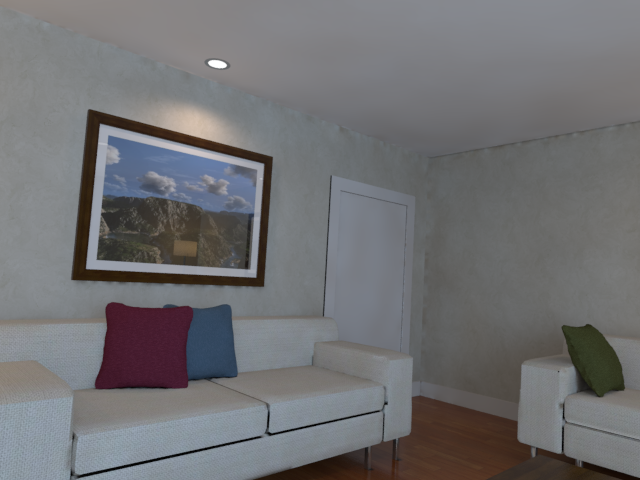
\includegraphics[width=\textwidth]{images/frame_000139.png}
                \caption{RGB image of frame 139 of lrkt2.}
                \label{sfig:frame1}
            \end{subfigure}
            \begin{subfigure}[b]{.48\textwidth}
                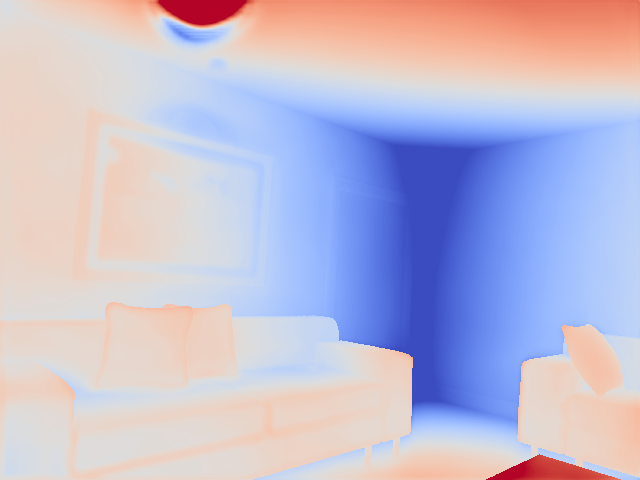
\includegraphics[width=\textwidth]{images/error_000139.png}
                \caption{depth error for frame 139 of lrkt2.}
                \label{sfig:error1}
            \end{subfigure}\\
            \begin{subfigure}[b]{.48\textwidth}
                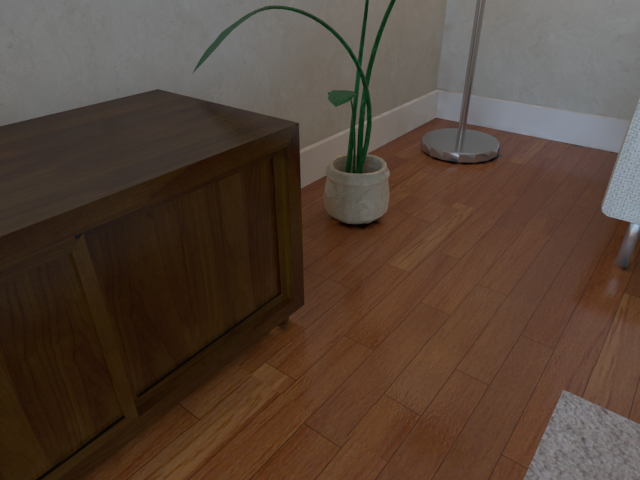
\includegraphics[width=\textwidth]{images/frame_000800.png}
                \caption{RGB image of frame 800 of lrkt2.}
                \label{sfig:frame2}
            \end{subfigure}
            \begin{subfigure}[b]{.48\textwidth}
                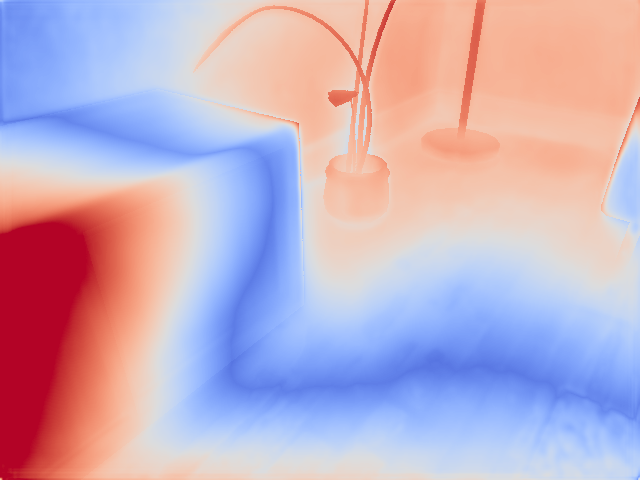
\includegraphics[width=\textwidth]{images/error_000800.png}
                \caption{depth error for frame 800 of lrkt2.}
                \label{sfig:error2}
            \end{subfigure}
            \caption{On the right side we visualize the error between our depth and the ground truth. Blue indicates that the area was estimated to be closer than they are, red indicates the area was estimated to be further away than it really is. The left side simply displays the corresponding RGB images.}
            \label{fig:depth_error}
        \end{figure}
        